\section{Wednesday for MAT4002}\index{Monday_lecture}
There will be a quiz on Monday.
\paragraph{Reviewing}
\begin{itemize}
\item
Connectedness / Path-Connectedness
\end{itemize}
\subsection{Remark on Connectedness}
\begin{proposition}\label{pro:4:14}
All path connected spaces $X$ are connected.
\end{proposition}
\begin{proof}
Fix any $x\in X$, for all $y\in X$, there exists a continuous mapping $p_y:[0,1]\to X$ such that 
\[
\begin{array}{ll}
p_y(0)=x,&p_y(1)=y.
\end{array}
\]
Consider $C_y=p_y([0,1])$, which is connected, due to proposition~(\ref{pro:4:9}).

Note that $\{C_y\}_{y\in X}$ is a collection of connected sets, and for any $y,y'\in X$, $C_y\cap C_{y'}\ni\{x\}$ is non-empty.
Applying proposition~(\ref{pro:4:10}), we imply $X=\cup_{y\in X}C_y$ is connected.
\end{proof}



\begin{example}
\begin{enumerate}
\item
Exercise: if $A\subset B\subset\overline{A}$, then ${A}$ is connected implies $B$ is connected. (Hint: $U\cap A=\emptyset$ implies $U\cap\overline{A}=\emptyset$.)
\begin{proof}
Suppose $B$ is not connected, i.e., for any open $U,V$ such that $B\subseteq U\cup V$ and $(U\cap V)\cap B = \emptyset$, we imply $U\cap B\ne\emptyset$ and $V\cap B\ne\emptyset$, and therefore
\[
\begin{array}{ll}
U\cap \overline{A}\ne\emptyset,
&
V\cap \overline{A}\ne\emptyset
\end{array}
\]
which implies
\[
\begin{array}{ll}
U\cap A\ne\emptyset,
&
V\cap A\ne\emptyset
\end{array}
\]
which contradicts to the connectedness of $A$.
\end{proof}
\item
The converse of proposition~(\ref{pro:4:14}) may not be necessarily true. Consider the so-called \emph{Topologist's bomb} example:
\begin{figure}[H]
\centering
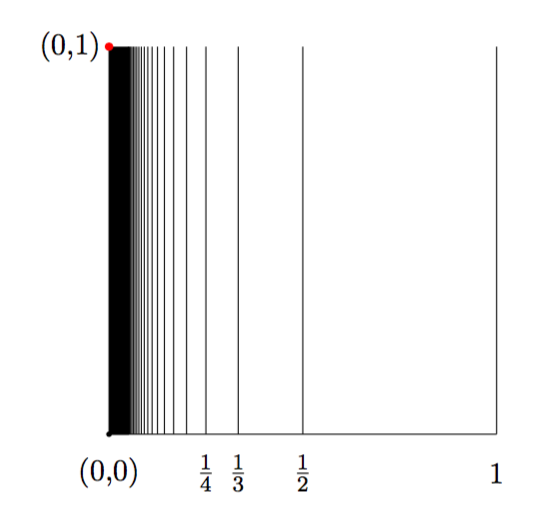
\includegraphics[width=0.6\textwidth]{week4/p_9}
\caption{Connected space $X$ but not path-connected}
\label{fig:4:1}
\end{figure}
Here we construct a connected space $X\subseteq\mathbb{R}^2$ but not path-connected shown in Fig~(\ref{fig:4:1}), i.e., the union of the interval $[0,1]$ together with vertical line segments from $(1/n,0)$ to $(1/n,1)$ and the single point $(0,1)$.
\[
X = ([0,1]\times\{0\}) \cup \bigcup_{n\ge1}(\{1/n\}\times[0,1])\cup(0,1).
\]
\begin{enumerate}
\item
Firstly, $X$ is not path-connected. We show that there is no path in $X$ links $(0,1)$ to any other point, i.e., for continuous mapping $p:[0,1]\to X$ with $p(0)=(0,1)$, we may imply $p(t)=(0,1)$ for any $t$.

Define 
\[
A=\{t\in[0,1]\mid p(t)=(0,1)\}.
\]
We claim that $A=[0,1]$, i.e., suffices to show $A$ is both open and closed in $[0,1]$:
\begin{enumerate}
\item
The set $A=p^{-1}(\{0,1\})$ is nonempty and closed, since the pre-image of a closed set is closed as well.
\item
The set $A$ is open: choose $t_0\in A$. By continuity of $p$, there exists $\delta>0$ such that 
\[\|p(t) - (0,1)\|=
\|p(t) - p(t_0)\|<\frac{1}{2},\quad
t\in[0,1]\cap(t_0-\delta,t_0+\delta).
\]
\qquad Since there is no point on the $x$-axis with the distance $1/2$ to the point $(0,1)$, we imply $p(t)$ is not on the $x$-axis when $t\in[0,1]\cap(t_0-\delta,t_0+\delta).$
Therefore, the $x$-coordinate of $p(t)$ is either $0$ or of the form $1/n$.

\qquad It suffices to show the open interval $I:=[0,1]\cap(t_0-\delta,t_0+\delta)$ is in $A$. Define the composite function $f=x\circ p: I\to\mathbb{R}$ , where the mapping $x:\mathbb{R}^2\to\mathbb{R}$ is defined as $(a,b)\mapsto a$.
Note that $I$ is connected, we imply $f(I)$ is connected, and $f(I)$ belongs to $\{0\}\cup\{1/n\}$.

\qquad The only nonempty connected subset of $\{0\}\cup\{1/n\}$ is a single point (left as exercise), and therefore $f(I)$ is a single point.
Since $f(t_0) = 0$,we imply $f(I) = \{0\}$, i.e., $I\subseteq A$. Therefore $A$ is open.
\end{enumerate}
\end{enumerate}
\end{enumerate}
\end{example}

\subsection{Completeness}
Compact set in $X$ is used to generalize ``closed and bounded'' in $\mathbb{R}^n$.
\begin{definition}
Let $(X,\mathcal{T})$ be a topological space.
A collection $\mathcal{U}=\{U_i\mid i\in I\}$ of open sets is an open cover of $X$ if 
\[
X=\bigcup_{i\in I}U_i
\]
A subcover of $\mathcal{U}$ is a subfamily
\[
\mathcal{U}'=\{U_j\mid j\in J\}, \quad J\subseteq I
\]
such that $\bigcup_{j\in J}U_j=X$.

If $J$ has finitely many elements, we say $\mathcal{U}'$ is a finite subcover of $X$.

We say $X$ is compact if any open cover of $X$ has a finite subcover.
\end{definition}

\begin{remark}
If $A\subseteq X$ has a subspace topology. then $A$ is compact iff 
for any open collection of open sets (in $X$) $\{U_i\}$ such that $A\subseteq\bigcup_{i\in I}U_i$, 
there exists a fintie subcover $A\subseteq\bigcup_{k=1}^nU_{i_k}$.
\end{remark}

\begin{proposition}\label{pro:4:15}
Let $X$ be a topological space.
The followings are equivalent:
\begin{enumerate}
\item
The space $X$ is compact
\item
If $\{V_i\mid i\in I\}$ is a collection of closed subsets in $X$ such that
\[
\bigcap_{j\in J}V_j\ne\emptyset,\quad \text{for all finite $J\subseteq I$,}
\]
then $\cap_{i\in I}V_i\ne\emptyset$.
\end{enumerate}
\end{proposition}
Compactness is an \emph{intrisical} property, i.e., we do not need to worry about which underlying space for this definition.
\begin{example}
\begin{enumerate}
\item
$X\subseteq\mathbb{R}^n$ is compact iff $X$ is closed and bounded. (Heine-Borel)
\item
Let $K\subseteq\mathbb{R}^n$ be compact, then define the set
\[
\mathcal{C}(K)=\{\text{all continuous mapping }f:K\to\mathbb{R}\}
\]
Note that the $d_\infty$ metric associated with $\mathcal{C}(K)$, say $\|f\|_\infty=\sup_{k\in K}f(k)$, is well-defined.

Under the metric space $(\mathcal{C}(K),d_\infty)$, any $\mathcal{J}\subseteq\mathcal{C}(K)$ is compact, if and only if $\mathcal{J}$ is closed, bounded, and equi-continuous. (Aresul-Ascoli)
\end{enumerate}
Therefore, we can see that the compactness is not equivalent to the closedness together with boundedness.
\end{example}

\begin{proposition}\label{pro:4:16}
Let $X$ be a compact space, then all closed subset $A\subseteq X$ are compact.
\end{proposition}
\begin{proof}
Let $\{V_i\mid i\in I\}$ be a collection of closed subsets in $A$ such that 
\[
\cap_{j\in J}V_j\ne\emptyset,\quad\text{for any finite $J\subseteq I$.}
\]
As $A$ is closed in $X$, we imply $V_j$ is closed in $X$.

Due to the compactness of $X$ and proposition~(\ref{pro:4:15}), we imply
\[
\cap_{i\in I}V_i\ne\emptyset
\]
By the reverse direction of proposition~(\ref{pro:4:15}), we imply $A$ is compact.
\end{proof}

\begin{remark}
Now consider the reverse direction of proposition~(\ref{pro:4:16}), i.e., are all compact subsets $K\subseteq X$ closed in $X$?

In general, the converse does not hold. Note that $K=\{x\}$ is compact for any topology $X$. However, there are some topologies such that $\{x\}$ is closed.
\end{remark}

In order to obtain the converse of proposition~(\ref{pro:4:16}), we need to obtain another \emph{separation axiom}:
\begin{proposition}\label{pro:4:17}
Let $X$ be Hausdorff, $K\subseteq X$ be compact, and $x\in X\setminus K$. 
Then there exists open $U,V\subseteq X$ such that 
$U\cap V=\emptyset$ and
\[
\begin{array}{lll}
U\cap V=\emptyset,
&
K\subseteq U,& x\in V.
\end{array}
\] 
\end{proposition}
\begin{proof}
Let $k\in K$, then by Hausdorffness, there exists open $U_k\ni k,V_k\ni x$ such that $U_k\cap V_k=\emptyset$.
Therefore, $\{U_k\}_{k\in K}$ forms an open cover of $K$. By compactness of $K$, $\{U_{k_i}\}_{i=1}^n$ covers $K$.
Constructing the set
\[
\begin{array}{ll}
U:=\bigcup_{i=1}^nU_{k_i},
&
V=\bigcap_{i=1}^nV_{k_i}
\end{array}
\]
gives the desired result.
\end{proof}
By making use of this separation axiom, we obtain the converse of proposition~(\ref{pro:4:16}):
\begin{corollary}
All compact $K$ in Hausdorff $X$ is closed.
\end{corollary}
\begin{proof}
For $\forall x\in X\setminus K$, by proposition~(\ref{pro:4:17}) there exists open $V$ such that $x\in V\subseteq X\setminus K$, and therefore $X\setminus K$ is open.
\end{proof}














